\documentclass[12pt]{article}

\usepackage[utf8]{inputenc}
\usepackage[T1]{fontenc}
\usepackage[english]{babel}
\usepackage{tabularx}
\usepackage{hyperref}
\usepackage[margin=2cm,a4paper,headsep=1.2cm]{geometry}
\usepackage{ifthen}
\usepackage{fancyhdr}
\usepackage{tikz}
\usetikzlibrary{arrows}
\usetikzlibrary{arrows.meta}
\usepackage{graphicx}


\renewcommand{\baselinestretch}{1.1}
\setlength{\parindent}{0pt}
\setlength{\parskip}{1em}

\setlength{\headheight}{1cm}
\setlength{\headwidth}{\textwidth}

\makeatletter
\newcommand{\labeltext}[2]{%
  \@bsphack
  \csname phantomsection\endcsname % in case hyperref is used
  \def\@currentlabel{#1}{\label{#2}}%
  \@esphack
}
\makeatother    

\newcommand{\prio}[1]{\ifthenelse{\equal{#1}{1}}{low}{\ifthenelse{\equal{#1}{2}}{medium}{\ifthenelse{\equal{#1}{3}}{high}{\textbf{INVALID!}}}}\relax}

\newcounter{fr}
\newcommand{\fr}[8]{
\refstepcounter{fr}\label{#8}
\begin{tabularx}{16cm}{l|X}
 & \textbf{#1} \hfill \textbf{FR\arabic{fr}} \\ \hline
Description & #2\\ \hline
\ifthenelse{\equal{#3}{}}{}{Precondition & #3 \\ \hline}
\ifthenelse{\equal{#4}{}}{}{Postcondition & #4 \\ \hline}
Rationale & #5
\ifthenelse{\equal{#6}{}}{}{\\ \hline Dependencies & #6} 
\ifthenelse{\equal{#7}{}}{}{ \\ \hline Priority & \prio{#7}}
\end{tabularx}
\vspace*{0.75cm}
}

\newcommand{\actor}[4]{
\labeltext{#2}{#1}
\begin{tabularx}{16cm}{|l|X|}
\hline 
Actor: & #2 \\
\hline
Description: & #3 \\
\hline
Representative: & #4 \\
\hline
\end{tabularx}
}

%\newcommand{\rref}[1]{\ref{#1}\textsuperscript{$\rightarrow$ p. \pageref{#1}}}
\newcommand{\rref}[1]{\ref{#1}}
\newcommand{\frref}[1]{FR\ref{#1}\textsuperscript{$\rightarrow$ p. \pageref{#1}}}
\newcommand{\nfrref}[1]{QR\ref{#1}\textsuperscript{$\rightarrow$ p. \pageref{#1}}}

\newcommand{\myrule}[1]{
	\begin{tikzpicture}
		\draw[{Diamond[open]}-{Diamond[open]}, ultra thick] (0,0) to (#1, 0);
	\end{tikzpicture}
}

\renewcommand{\contentsname}{Table of Contents}

\begin{document}

% title page 
\begin{titlepage}

	\centering 
	\scshape 
	\vspace*{\baselineskip}
		
	\myrule{\linewidth}	
	\rule[1\baselineskip]{0.95\textwidth}{0.4pt}
    
    \Large
    Requirements engineering
    \normalsize
   

	\rule[-1\baselineskip]{0.95\textwidth}{0.4pt}
	\myrule{\linewidth}
	
	\vspace{2\baselineskip}

    Flutter smart sensing library \\ for medical and psychological study apps
	
	
	\vspace*{15\baselineskip}
	
	edited by
	
	\vspace{0.55\baselineskip}
	
	{\scshape Leonhard Alkewitz, Florian Gebhardt, Hermann Fröhlich, \\ Mukhtar Muse, Felix Schlegel}
	
	\vspace{0.55\baselineskip}
	
	\vfill
	
\end{titlepage}


% table of contents
\tableofcontents
\thispagestyle{empty}

\newpage

% configure header and footer
\pagestyle{fancy}

\fancyhead[R]{\thepage}
\fancyhead[L]{\leftmark}
\fancyfoot{}

\section{Adding a new Feature/User Story}
\subsection{Creating a new User Story}

To add a new feature, it is important to understand the user story process from the perspective of the user. User stories are a proven method to describe requirements from the user’s perspective. Therefore, the needs of the user should be considered when creating a user story.

Once the user story is clearly formulated, you can move on to the next step and integrate it into an existing user story map. To do this, you should first identify the right place in the existing system where the new function can best be integrated. Then add the user story to the user story map by creating a new entry or updating an existing one that describes the feature and its requirements.

Integrating the user story into the map gives users a clear understanding of how the new feature fits into the overall system and how it can be used. This can help them make informed decisions and use the new feature effectively.

It is important to remember that integrating a new user story into a map may also require changes to other parts of the system. It is therefore important to carefully plan and coordinate the integration of new functionality to ensure that it fits seamlessly into the existing system.

 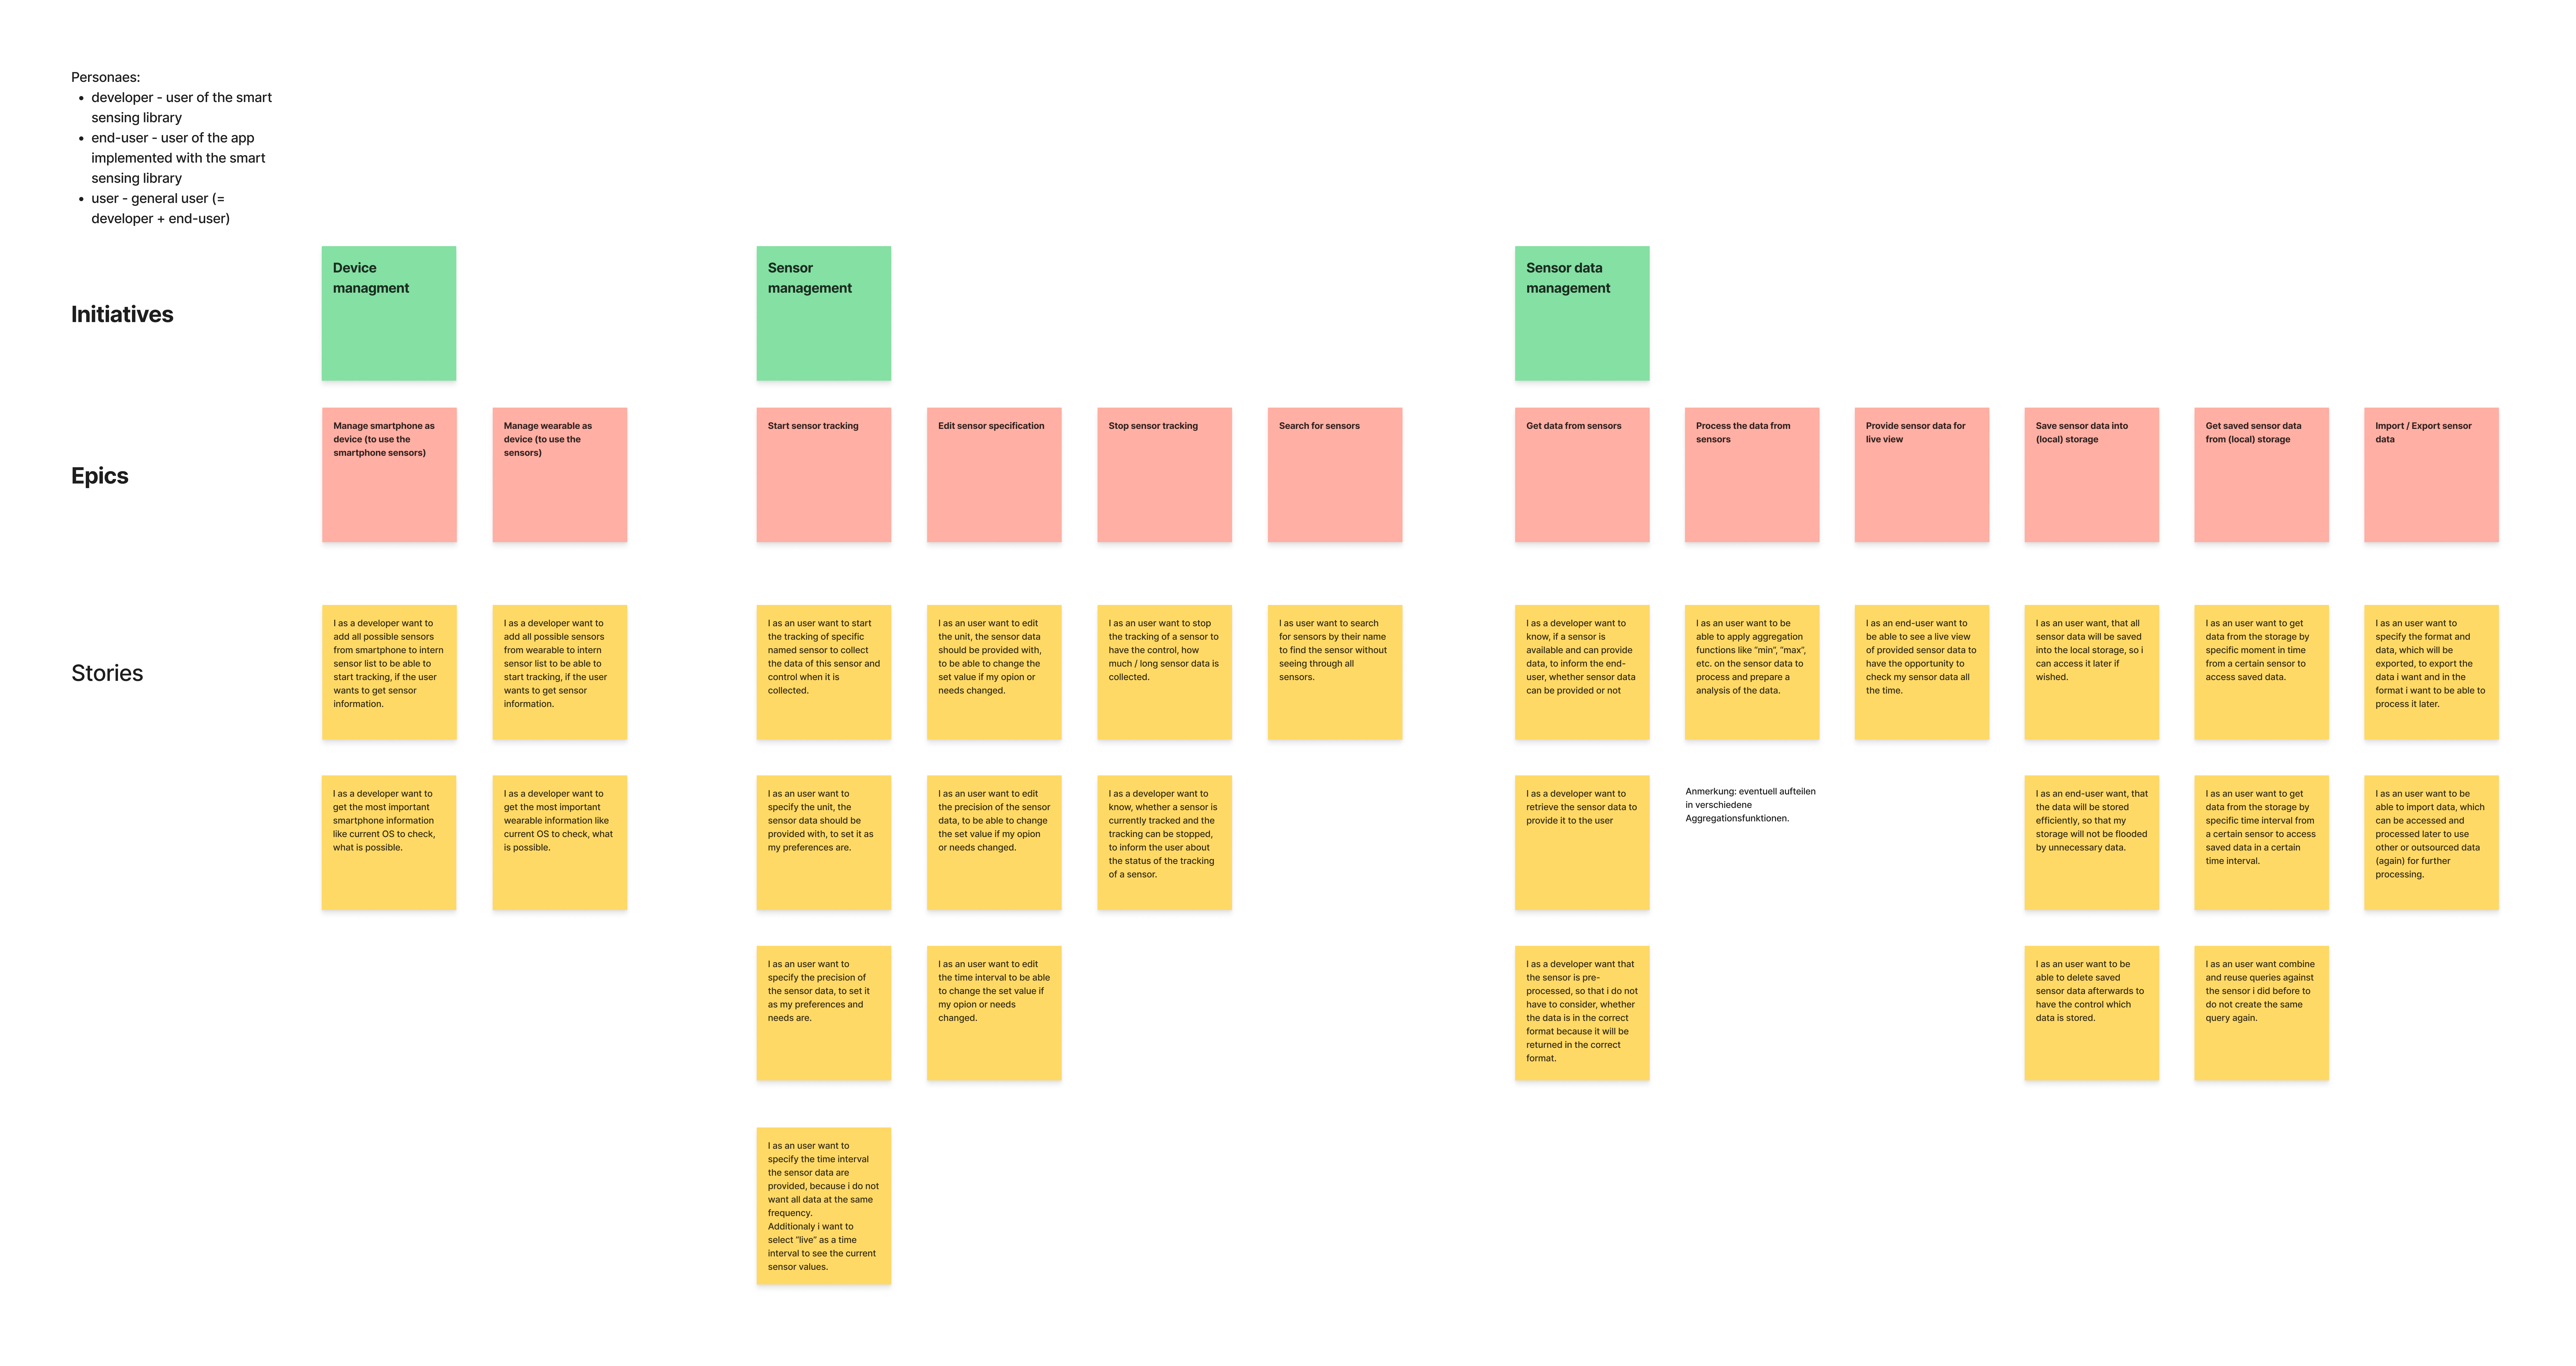
\includegraphics[width=\textwidth]{user_story_map.png}
 

\subsection{Adding a new Feature}

To add a new feature, the whole process takes place within our \href{https://gitlab.uni-ulm.de/se-anwendungsprojekt-22-23}{GitLab environment}
You can then create an issue. An issue is used to describe the new feature or desired functionality in terms of a specific task that needs to be implemented.

After the issue is created, a separate feature branch is created for the feature. All changes and developments take place in this separate feature branch to isolate the development of the feature from other changes in the main branch. This allows developers to work on the new feature without affecting the stability of the main branch and ensures that the new feature can be thoroughly tested before being merged into the main branch.

\subsubsection{Creating an Issue}
When creating the issue, you should use the appropriate template to clearly define the objective of the feature. 

For example, if you want to add a new sensor to the app, you can select the Issue Feature option and fill out the template with the relevant information. The template includes sections for feature description, use case, benefits, requirements, and links/references. 
 \begin{enumerate}
      \item
      In the feature description section, you can explain what type of sensor you want to add and how it should function. 
      \item
      In the use case section, you can describe how the new sensor will be used by users. In the benefits section, you can explain how the new sensor will improve the app and provide value to users. 
      \item
      In the requirements section, you can list any technical or functional requirements that must be met for the new sensor to work properly. 
      \item
      Finally, in the links/references section, you can provide any relevant links or references that may help developers understand your requirements and implement the new feature accordingly. 
      

    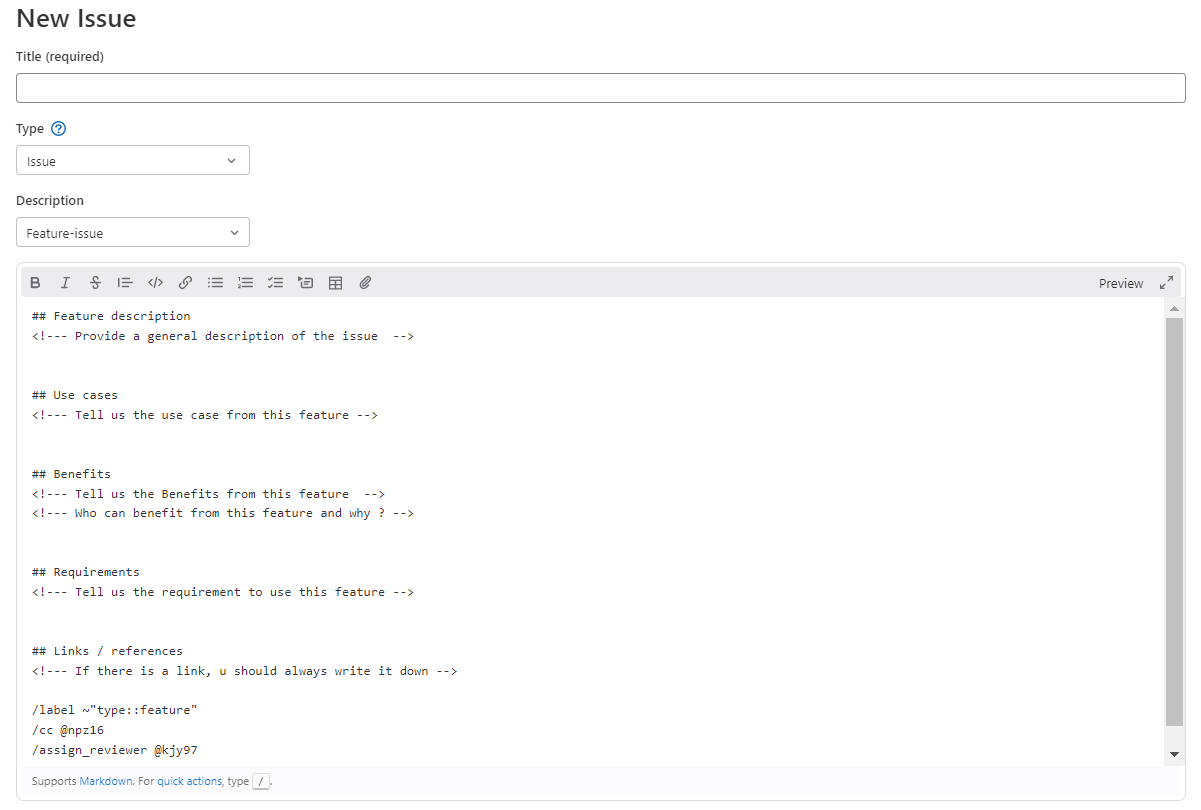
\includegraphics[width=0.9\textwidth]{issue.png}
  
 \end{enumerate}

In addition to this, you should consider who should be selected as the assignee for the issue, be it yourself or another person responsible for implementing the feature. Assigning an assignee clearly establishes responsibility.To further specify the issue and place it in the overall context of the project, you can define an Epic and a Milestone, if available. 

An Epic summarises related features or tasks and allows for better organisation and prioritisation .A milestone helps track the progress of the project and mark important stages.

In addition, you can add a predefined label to further mark the issue and make it easier to identify. This makes it easier to filter and categorise issues within the project management system.

To plan and track the progress of the issue, it is useful to set a date by which the issue should be completed. You should also specify the sprint iteration in which the issue is to be worked on. This allows for effective planning and coordination of workflows within the development team.

By including this additional information and details, the issue becomes more comprehensive and structured. This facilitates communication, planning and progress of the feature in the project.

 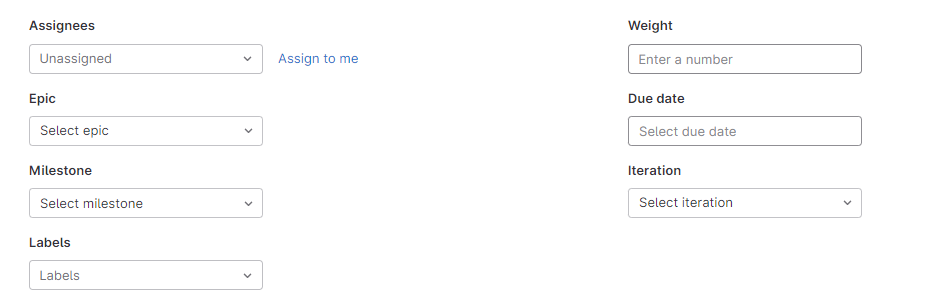
\includegraphics[width=\textwidth]{issue2.png}
 
\subsubsection{Reviewing an Issue}
\begin{minipage}[t]{0.51\textwidth}
As soon as the development of the feature is completed, a so-called merge request is created.

In this merge request, the completed issue is submitted for review by another developer. 

The reviewer checks the code, the functionality and the implementation of the feature. 

In the process, possible problems, improvement requests or questions are discussed in the form of threads within the merge request.

The merge request remains open until all threads have been successfully processed and resolved. Once the reviewer is satisfied and all open issues are resolved, he can approve the merge request. This merges the issue into the main branch and integrates the new feature into the overall system.

This structured approach ensures that all changes and developments are thoroughly reviewed and discussed before they enter the main branch. This ensures the quality and stability of the system and potential errors or inconsistencies can be identified and corrected at an early stage.


\end{minipage} 
\hfill
     \begin{minipage}[t]{0.55\textwidth}
        \vspace{-\baselineskip}
        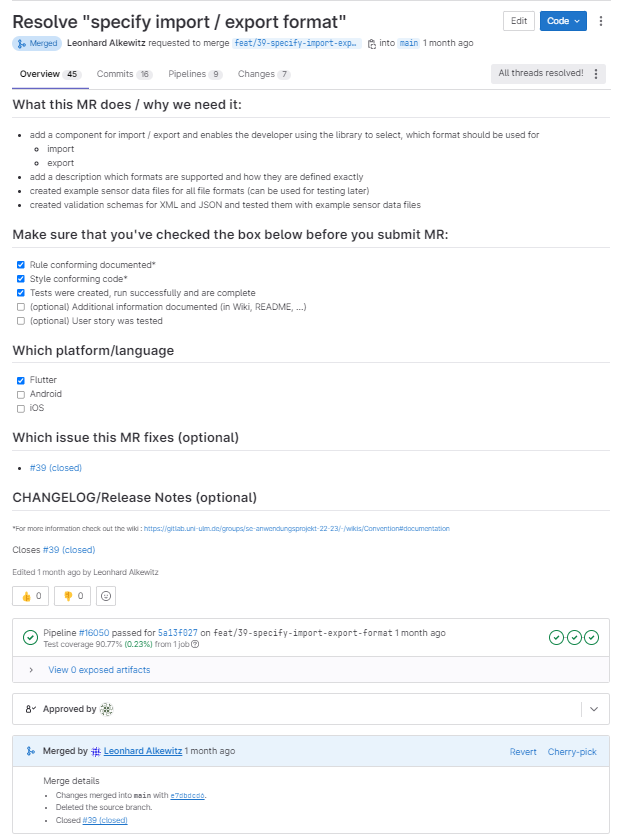
\includegraphics[width=\textwidth]{mr.png}
    \end{minipage}
    
    All in all, each feature is developed in its own feature branch, goes through the merge request process with reviews and discussions before it is finally merged into the main branch. In this way, we ensure effective collaboration and controlled integration of new features into the overall system.
\subsubsection{Weight of Issues}
The weighting of an issue is done in our regular sprint meetings, which are held every two weeks. In these meetings, we discuss together how an issue should be weighted. The weight of an issue indicates the estimated effort required to complete it within a sprint. We use a scale of 1 to 5, with a value of 1 representing the lowest and least effort, while a value of 5 signals the highest and greatest effort.

Through this structured approach, we can estimate the workload for each sprint and ensure that new features and user stories are integrated into our system effectively and professionally. This allows us to continuously improve the user experience and meet the needs and requirements of our users.

\section{Decisions about adding/removing features or user stories}
When it comes to adding or removing a feature, this is also discussed in the sprint meeting and then decided. It happens that certain features have to be removed, either because they cannot be implemented within the given time frame or due to a lack of capacity. In such cases, we may need to prioritize other features and remove those that are less important or require more effort to implement. It is the same with the integration of features. We have found that in some cases we were missing certain functionalities of which we had no prior knowledge and which had to be added subsequently.

Through this structured approach, we can effectively manage our workload and ensure that we are able to deliver high-quality features within the given time frame.

\end{document}
